\section{System Architecture}

Our first step, after reading the description of our project, was to decide what kind of application or system would be best suited to tackle our requirements. The first thing that we gleaned from the specification was that some form of persistent storage would be required. For example, the user submitted scripts must be stored so that they can later be raced against new scripts and data used to rank the scripts must be recorded so that a leaderboard can be shown. It was also mentioned in our project's specification that we should use the Unity game engine for the physics simulation and visualisation of our vehicle races. These two requirements gave us a solid starting point for designing our system. Our first thought was to develop a stand alone Unity application to run on any desktop machine. This option would have required one machine to act as a server and manage the centralised data while the other machines communicate with it using networking code inside of Unity. It would also have meant we'd need to build a full user interface for uploading, editing and managing scripts inside of Unity. The more we thought about this the more we realised that these tasks would be a massive undertaking and highly difficult to achive in the time frame, due to our group's limited knowledge of Unity.

Once we began thinking about alternatives an obvious solution sprang to mind. A huge benifit of Unity is that it is highly portable and can be run on many different platforms. One of these platforms is the Unity Web Player, a browser plug-in that allows Unity applications to be run inside all modern web browsers. If we used the web player we would could pull all of the things that are difficult to do in Unity outside of the Unity application and into the web browser. Thus turning the task of creating an easy to use interface for uploading scripts into a web design problem, a domain that is a lot better suited to solve user interface tasks such as this. The Unity application is then only needed for running and visualising the races. Unity also provides features for communication with the web browser, in both directions, when running in the web player, making passing data to the Unity application at runtime easy. This design also reduces the complexity of the networking problems as now one machine can run a web-server and database, using standard web technologies, while client machines simply run a web browser, containing the Unity Web Player, and communicate with the server using standard web protocols.

\subsection{Component Diagram}

\tikzset{%
  block/.style    = {draw, thick, rectangle, minimum height = 3em, rounded corners,
    minimum width = 3.5em, align=center},
  sum/.style      = {draw, circle, node distance = 2cm}, % Adder
  %input/.style    = {coordinate},
  db/.style  = {draw, cylinder, shape border rotate=90, aspect=0.25},
  interface/.style    = {draw, thick, rectangle,
    minimum width = 4em, align=center},
}

\begin{center}
\begin{tikzpicture}[auto, thick, node distance=2cm, >=triangle 45]
	% Blocks of FRONT END:
	\draw
		node at (1, -1.7) [block] (unity) {Game \\ Objects}
		node [block, right of=unity, right=-0.25cm] (webplayer) {Unity \\ Webplayer}
		node [block, right of=webplayer, right=-0cm] (unityscript) {Unity \\ Script}
		node [block, right of=unityscript, right=-0.35cm] (ai) {AI\\Script}
		node [block, right of=ai, right=-0.5cm] (browser) {Browser}
		%node [sum, right of=input1] (suma1) {Unity}
	;
    	% Joining FRONT END:
	\draw[->] (browser) -- node {} (ai);
	\draw[->] (ai) -- node {} (unityscript);
	\draw[->] (unityscript) -- node {} (webplayer);
	\draw[->] (webplayer) -- node {} (unity);
	\draw[-] (webplayer) |- node[right=3.5cm, above] {\small Request Commands } ($(browser.north) + (0, 0.5)$);
	\draw[->] ($(browser.north) + (0, 0.5)$) -- node {} (browser);

	% Blocks of MIDDLE
	\draw
		node at (5.5,-4) [block, name=rest] {REST API}
	;

        % Blocks of BACK END
	\draw
	        node [block, below of=unity, below=2.3cm, name=express] {Express\\Router}
	        node [block, right of=express, right=0cm, name=passport] {Passport \\ Auth.}
	        node [db, below of=passport, below=0cm, name=mongo] {MongoDB}
	        node [interface, above of=mongo, above=-1cm, name=monk] {Monk Adapter}
	        node [block, right of=passport, right=0cm, name=routes] {Routes}
	        node [block, right of=routes, right=0cm, name=views] {Views}
	;
	% Joining BACK END
	\draw[->] (express) -- node {} (passport);
	\draw[->] (rest) -| node {} (express);
	\draw[->] ($(browser.south) + (-0.2, 0)$) |- node[left=2.25cm, below] {\small Request Page} (rest);
	\draw[-, dotted] (passport) -- node[below right] {} (monk);
	\draw[-] (monk) -- node {} (mongo);
	\draw[->] (passport) -- node {} (routes);
	\draw[->] (routes) -- node {} (views);
	\draw[-, dotted] (routes) |- node {} (monk);
	\draw[->] (views) -| node {} ($(browser.south) + (0.2, 0)$);

	% Boxing
	%\draw [color=gray,thick, dotted] ($(passport.north west)+(-0.2,0.2)$) rectangle ($(monk.south east)+(0.2,-0.2)$);
	\draw [color=gray,thick](-0.5,-3) rectangle (12.55,0);
	\node at (-0.5,0) [above=5mm, right=0mm] {\textsc{Front-End}};
	\draw [color=gray,thick](-0.5,-10.5) rectangle (12.55,-5);
	\node at (-0.5,-10.5) [below=5mm, right=0mm] {\textsc{Back-End}};
\end{tikzpicture}
\end{center}

\section{Back-end {\color{green} BEN}}

The design of our back-end was focused around a simple REST API, while the implementation primarily involves NodeJS and its supporting libraries:
	\begin{itemize}
	        \item Express
		\item Passport (passport-local)
		\item Monk
	\end{itemize}

\subsection{REST API}
Why use REST API?

Below you can see some example interactions with our REST API:\\

\begin{center}
\begin{tabular}{| l | l | l | l |}\hline
Route & Request &  Response & Explanation\\\hline\hline
/script & GET & View & Show the create new script page\\\hline
/script & POST & None & Store a new script to the server\\\hline
/script/DrEvil & GET & String & Get the code for script DrEvil\\\hline
/edit/DrEvil & GET & View & Show the live edit script page\\\hline
/tournament & GET & View & Show the next tournament match\\\hline
/tournament & POST & View & Store the match result and show the next \\\hline
\end{tabular}
\end{center}

Comment on the table.

\subsection{MongoDB}
Why use MongoDB?

Although MongoDB is a non relational database, we can still model the data storage as such:

\begin{center}
\begin{tikzpicture}[node distance=7 em]
\node [entity] (person) {User};
\node [relationship] (has) [right of=person] {Owns};
\node [entity] (script) [right of=has] {Script};
\node [attribute] (email) [above of=person] {\key{Email}} edge (person);
\node [attribute] (pid) [below of=person] {Year?} edge (person);
\node [attribute] (pid) [below left of=person, above=0cm] {Degree?} edge (person);
\node [attribute] (pid) [left of=person, left=-0.6cm] {University?} edge (person);
\node [attribute] (pid) [above left of=person, above=-0.5cm] {Hash} edge (person);
\node [attribute] (pid) [above of=script] {\key{Name}} edge (script);
\node [attribute] (pid) [below of=script] {Code} edge (script);
\node [attribute] (pid) [above right of=script] {Language} edge (script);
\node [attribute] (pid) [below right of=script] {Rating} edge (script);
%Edge
\path[every node/.style={font=\sffamily\small}] (person) edge node [above] {0..N} (has);
\path[every node/.style={font=\sffamily\small}] (script) edge node [above] {1..1} (has);
\end{tikzpicture}
\end{center}

\subsection{Risks}
Anticipation \& Mitigation

\subsection{Challenges}
Solutions

\section{Browser Front-End {\color{red} TOM}}

For the browser front-end, i.e. website, we used three technologies : Jade, Bootstrap and the Ace editor.


\subsection{Jade}
As explained above, we chose to use the Node.js platform, and we next had to chose a template engine for it's web template system. We chose to use Node's default engine, Jade, which is written in JavaScript and specifically a templating language for HTML. It simplifies writing web pages as it is less verbose than HTML, and allows template inheritance (demonstrated below) alongside other dynamic constructs such as conditionals and loops.
\vspace{-2mm}
\begin{figure}[H]
\centering
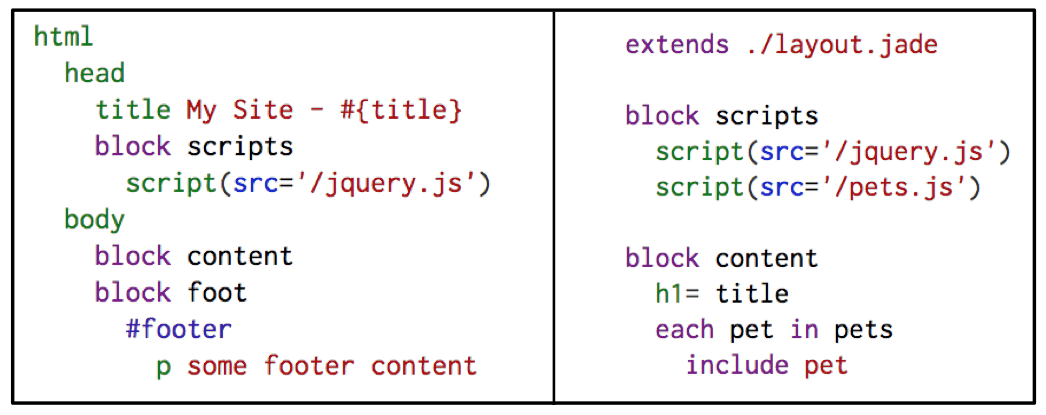
\includegraphics[scale=0.25]{jadeexample.png}
\caption{Jade template inheritance is simple and powerful.}
\end{figure}

\noindent Compared to other engines such as Swig and Hamljs, which have similar feature sets, Jade has had reported sluggish benchmarking performance \cite{benchmarks} (obviously some benchmarks can't be treated as gospel). However, performance was not a concern for us; templating engines are very rarely a system bottleneck, and the decision to use Jade was founded upon it's usability and readability.

\subsection{Bootstrap}
Given our limited experience using Jade/HTML and CSS, alongside our negligible artistic talent, we opted to use Twitter's Bootstrap to design our website. Bootstrap makes web design a breeze by providing the HTML and CSS templates for well-designed web components, including forms, buttons, navigation bars, JavaScript extensions and more. In particular, we used the Sandstone\cite{sandstone} template from Bootswatch (released under MIT license), demonstrated in the figure below. Although this may not give users with a particularly unique experience, it means providing users with a familiar experience that would allow them to utilise preconceived assumptions on how the website can be navigated - avoiding the need to explain the website explicitly.

\begin{figure}[H]
\centering

\includegraphics[width=0.5\textwidth]{sandstonetheme.png}
\caption{Bootswatch Sandstone theme sample.}
\end{figure}

\subsection{Ace}
Apart from the most cavalier advocates of text editors, programmers shudder at the idea of coding in a plain text area. To simplify the process of reading, writing and submitting scripts, we chose to use a web-based code editor. There are few open-source editors that can rival the performance, features and simplicity of Ace (a standalone editor written in JavaScript). Ace is actively developed for use in the online Cloud9 IDE, yet can be embedded in any web page (see picture below) given its BSD license.

\begin{figure}[H]
\centering
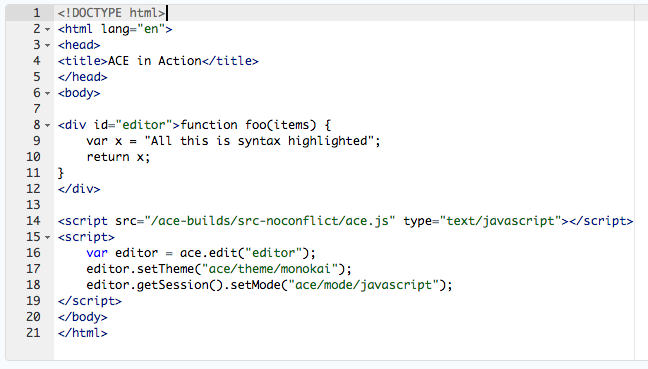
\includegraphics[width=0.75\textwidth]{aceeditorexample.png}
\caption{Ace editor containing code needed to embed in a web page.}
\end{figure}

\noindent By using Ace, users have JavaScript syntax highlighting, syntax error checking, searching/replace, automatic indentation etc. Not only does this improve the productivity of a user, which is important given the time pressures which may be faced if a queue forms at the G-Research careers fair stand; but it provides immediate feedback for those unfamiliar with JavaScript syntax, which may be the majority of users, reducing the likelihood of submitting broken scripts.

\subsection{Risks}

\subsubsection{Browser Cross-Compatibility}

It is rare for websites and web applications to function identically or appear the same across multiple web browsers, due to the varying compatibilities of even the most popular browsers - this can be problematic for many modern websites. We mostly spent time testing AI Racing Market on Google Chrome, yet tested on Mozilla Firefox and Safari occasionally. Needless to say, this does not replace proper cross-browser compatibility testing using the many tools (such as emulation environments) available to developers these days. However we did not deem this a significant risk, as G-Research employees should be able to iron out compatibility issues prior to a careers fair, installing and choosing the most functional browser in advance. With most of the well known browsers, it is likely that the user interface will simply appear jumbled yet remain functional.

\subsection{Challenges}
Solutions

\section{Unity Application {\color{blue} CHRISTOPHE}}
No external tech used except for a few of Unity's basic script assets, e.g. smooth follow cam.

Main design points:
Designing the Script API
Managing and recording race data e.g. checkpoints, hud
Comunication with browser i.e. starting race, where scripts are exectued, how many calls per frame

Unity applications are based around a system of scenes that can be switched between at runtime. We used this in our application to have a seperate scene for each racetrack we had built. As, in our case, each time the application is loaded only

\subsection{API Design}
The key component of the Unity application is the scripting API and our first step in its design was to decide how to give information about the race track so the user can complete a lap. We eventually settled on making this very simple for the user - we drew a line along the centre of the track and let the user set the speed of the car. Our API will then automatically steer the car along the centre line at the set speed. Our reasoning on making steering so simple was that guiding the car around the track is the first and least interesting step and we did not want every user to spend the first few minutes writing the same line following script. However, a race will disintegrate into a train of cars driving around the track if all cars follow the same line, the first car in the train at the start of the race will be the winner. We solved this creating two more lines for the cars to follow on either side of the centre line and providing API calls to switch to the line on the left or on the right. These calls can be used to overtake cars or to switch to the inside line of a corner.

Finally, we added a few more features which scripts can use to distinguish themselves: the distance to the next corner, the curvature of that corner and a ``boost'' ability which gives the car a large speed increase but may only be used every few seconds. A good script can make use of these features by boosting along straight sections and slow down according to the sharpness of the corner. Our test scripts have shown these features work well at differentiating scripts as scripts which use the boost and variable speed are much faster than scripts which can only change lines.

\subsection{Race Data}

\subsection{Browser Communication}

\subsection{Risks}
Spending ages on

splines from timeboxed spikes section?

Anticipation \& Mitigation

\subsection{Challenges}
Designing the script API

Initially we had a very simplistic system of controlling and receiving environment information from the car.

steering and throttle control for control. Proximity sensors (ray casting) for position information.

Solutions

\subsubsection{Steering the Car}
To guide the car around the track we initially placed invisible walls along the edge of the track and created proximity sensors on either side of the car to measure the distance to these walls. The output of the sensors was used to steer the car toward the current lane. The main problem with this approach was that the cars would always drive forward even when pointing the wrong way after skidding or a crash causing the cars to drive the wrong way around the track.

We solved this problem by replacing the walls and proximity sensors with a spline along the centre of the track and keeping a target position on this spline. The car will always steer toward this target position and the target will always be a small distance in front of the car. This ensures that the car will always drive the right way along the track. Another advantage of the splines is that if two cars take a corner too quickly, the car moving moving faster will end up further from the track and therefore lose more time than the slower car. With the old approach, both cars would have simply bounced off the walls and the slower car would have no advantage.

\section{User Interface Design {\color{red} TOM}}

\subsection{Design Philosophy}

At a a busy careers fair we expect students will have roughly 5-10 minutes sessions with AI Racing Market. Ideally students will have the chance to return and improve their scripts, yet this may be infeasible if there are a lot of interested students. Given students will be short on time, under pressure and likely new to the game, we focused on :
\vspace{-1mm}
\begin{enumerate} \itemsep -2pt 
\item Simplicity
\item Minimal Interactions
\end{enumerate}

We previously justified our use of Bootstrap by the provision of a familiar user experience. By providing the user with a simplistic and familiar interface, users need little explanation of website navigation and can simply focus on script editing and submission. 

An example of how we achieved this was a common navigation bar seen on each web page. This functions as a website backbone, providing the user with access to all of the website's  features. Our template engine, Jade, made this incredibly simple (as shown below); we wrote a basic navigation template that extended our generic Bootstrap layout, which could then be included within the other templates (in Node.js, these are called {\it views}). 

\begin{figure}[H]
\centering
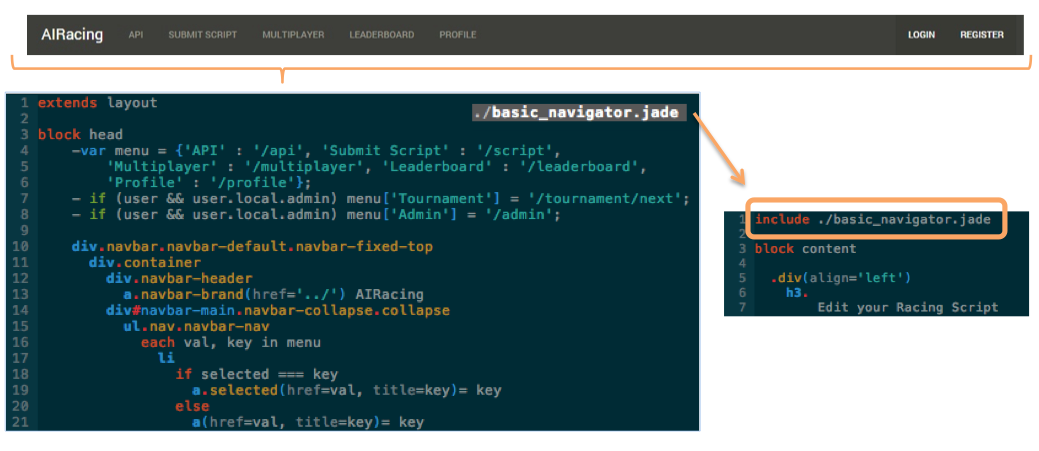
\includegraphics[width=\textwidth]{jadenavigator.png}
\caption{Jade navigator template included within each view.}
\end{figure}

\subsection{Responsive Script Editing}

\begin{enumerate}
\item Iterative development - for collaboration with G-Research
\item Immediate feedback - otherwise scripts submitted and left in the ether until tournament
\end{enumerate}

\subsection{Anonymous Script Submission}

\begin{enumerate}
\item Users dont need to register, submit straight after notes on handout
\item Associated with script name, no need to feel like G-Research will judge 
\end{enumerate}

\subsection{Admin Features}

\begin{enumerate}
\item Ed wanted us to restrict access to multiplayer/leaderboard - they alter ELO
\item Unrestricted REST endpoints
\end{enumerate}

\section{Script Execution and Sandboxing TODO {\color{green} BEN}}
How did we convert javascript to unity script?
How do we allow global state?
Challenges to overcome: no objects. Direct control over unity objects, e.g. car teleportation. Allowing other languages.
Risks: Dr Evil!!

\section{Harvesting Personal Data TODO}
One of the primary objectives of our project is the acquisition of personal data about potential employees. This includes information such as email address, university degree, etc.
\subsection{Non-invasive authentication}
We don't want to scare users away to early...
Allow anonymous script posting..
\subsection{Risks}
We must avoid leaking personal data...
For example, when designing our leaderboard we had to bare in mind we didn't want to display user's emails to passing strangers...


